\subsection{Asymmetric CubeRootMerge and SquareRootMerge}
\label{sec:root-merge-evaluation}

We additionally implement the two asymmetric merge constructions.
For each long-list size $n=2^{10},2^{11},\ldots,2^{20}$, we set the short-list
length to $m=\lceil n^{1/3}\rceil$ for CubeRootMerge and
$m=\lceil\sqrt n\rceil$ for SquareRootMerge.
Each construction is compared with Batcher on exactly the same $(m,n)$ input
dimensions. These experiments measure the asymmetric building blocks separately
from the balanced, recursively composed \ourprotocol\ experiments above.

\paragraph{Implementation and setting.}
All implementations use 32-bit unsigned keys and return XOR shares of the
stable gather permutation of the concatenated inputs. Ties put the short list
first and preserve each list's order. We use the same real two-party,
semi-honest GMW and OT/VOLE backend as above, with its default 128-bit security
parameters and fresh private randomness
and correlations for every execution. The new protocol implementation and API
occupy 682 physical lines of C++, excluding the benchmark driver
and inherited primitives. The artifact records exact source and executable hashes.
The library also supports keys up to 256 bits; these wider keys are tested for
correctness but are not included in the timing comparison.

Experiments use the Lenovo 83DF laptop described above. Its Intel Core
i9-14900HX processor has 32 logical cores. The laptop has approximately
32\,GiB physical RAM, running
Ubuntu under WSL2 with approximately 15\,GiB guest RAM.
The release build uses GCC~13.3, \texttt{-O3}, and \texttt{-march=native}.
Local execution schedules both parties on one OS thread. TCP execution uses
one process per party, each with two Asio I/O workers and a main thread;
no GMW worker pool is enabled. CPU affinity and frequency are not fixed.
We use $2^{20}$-entry correlation batches and concurrency two for every method.
Setup, preprocessing, and online execution are timed separately.
Reported offline-plus-online totals exclude local circuit construction;
its time is recorded separately in the artifact.
The public synthetic inputs are identical within each matched repetition;
opening the output for oracle verification occurs after timing.

The Batcher baseline is an odd--even merge network for the exact unequal
lengths, with empty recursive branches removed using public dimensions.
It does not enlarge the shorter list to length $n$.
Comparators include the original index as a tie breaker, and the final layer
retains only the index bits. This unequal-length baseline is distinct from
the balanced bitonic network used in the earlier tables.

\paragraph{Concrete refinements.}
Both root constructions partition the long list into public blocks of size $b$.
The final partial block is padded with an extra-bit positive infinity.
We compare against block maxima, assign equal keys to the first qualifying
block, and send keys above the long-list maximum to its last block.
First occurrences select real blocks and repeated occurrences select dummies.
A joint shuffle opens a fixed multiset consisting of $m$ distinct selection
tags and a public number of zeros. Thus, the number and locations of distinct
selected real blocks remain hidden.

CubeRootMerge retains dummy holes and gates their comparisons off. It performs
two all-pairs passes, with $m(\lceil n/b\rceil-1)+m^2b$ key comparisons.
Secret prefix counts of selected blocks correct insertion ranks for the
unselected blocks. SquareRootMerge instead uses secret prefix copying to give
each short-list key its selected block, then performs
$m(\lceil n/b\rceil-1)+mb$ comparisons. A segmented suffix sum recovers the
long-list insertion counts. We flatten scan work across tree edges and count
words to reduce GMW padding at narrow tree levels. Boolean carry circuits
implement additions; these are included in the measured cost and depth.

Both constructions restore long-list positions by unshuffling narrow count
corrections instead of entire key blocks. The forward and inverse routing
reuse the hidden permutation with disjoint fresh masks. A separate joint
shuffle inverts the final secret ranks to a gather permutation.
The online depth bound sums executed GMW AND layers and nine one-way steps for
shuffling, tag opening, reverse routing, and final extraction.
It is a concrete dependency bound, not a packet count or the idealized
primitive-round count in the theoretical construction.
The correctness suite passes 198 real-cryptography executions with random
XOR shares, including duplicates, both disjoint orders, irregular dimensions,
block overrides, and wide keys. A plaintext model additionally passes 13,504
root-protocol cases and exhaustive unequal-Batcher binary inputs on small sizes.

\paragraph{Public parameter tuning.}
For each size, let $b_0$ be the smallest power of two at least $m$.
We consider $b_0/4,b_0/2,b_0,2b_0$, clipped to valid positive powers of two,
and minimize estimated online payload bytes, including padded GMW gates,
block routing, and rank inversion. The model excludes transport framing;
ties favor lower depth. This selection uses only public circuit parameters,
not key values or the fastest measured trial. All candidate schedules are
retained. Table~\ref{tab:root-parameters} lists the choices, which remain fixed
across repetitions and network profiles.

\begin{table}[!htbp]
\centering\small
\begin{tabular}{rrrrr}
\hline
$\log_2 n$ & Cube $m$ & Cube $b$ & Square $m$ & Square $b$ \\
\hline
10 & 11 & 8 & 32 & 16 \\
11 & 13 & 8 & 46 & 32 \\
12 & 16 & 16 & 64 & 32 \\
13 & 21 & 16 & 91 & 64 \\
14 & 26 & 32 & 128 & 64 \\
15 & 32 & 32 & 182 & 128 \\
16 & 41 & 32 & 256 & 128 \\
17 & 51 & 64 & 363 & 256 \\
18 & 64 & 64 & 512 & 256 \\
19 & 81 & 64 & 725 & 512 \\
20 & 102 & 128 & 1024 & 512 \\
\hline
\end{tabular}

\caption{Public list dimensions and block sizes for the asymmetric evaluation.
Batcher uses the same $(m,n)$ dimensions and has no block-size parameter.}
\label{tab:root-parameters}
\end{table}

\paragraph{Scaling results.}
We take three fresh executions per method, shape, and size, alternating
protocol order. Communication sums both parties' sent bytes.
Figures~\ref{fig:root-communication} and~\ref{fig:root-local} show every tested
power of two; time markers are medians and error bars are observed ranges.
Ratios below one favor the root construction. We report online and offline
costs separately because lower online communication does not imply lower
preprocessing communication or a consistent local speedup.
Both root constructions communicate fewer online bytes at every tested size.
They also have lower local online medians at every tested size from $2^{17}$
onward. At the smaller sizes, local timing differences are non-monotone;
the complete curves and observed ranges are therefore shown rather than
assigning a universal time crossover.

\begin{figure}[!htbp]
\centering
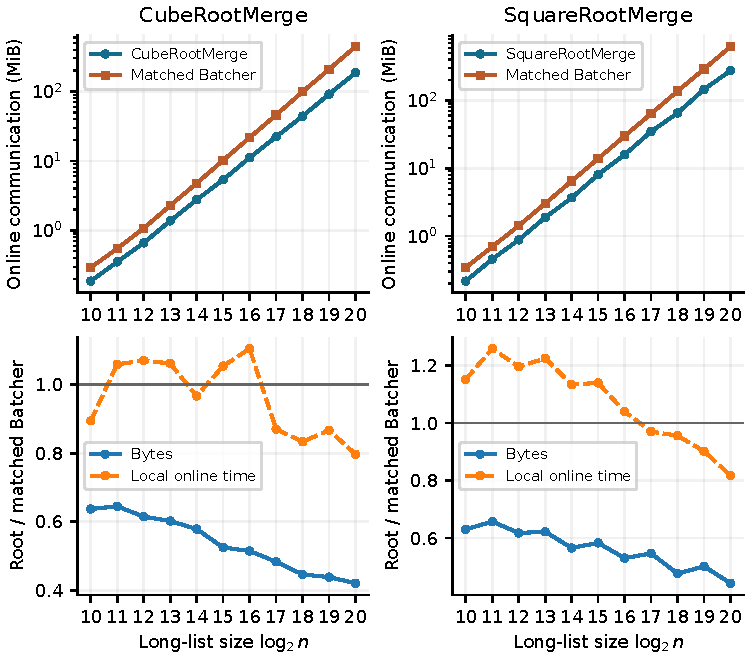
\includegraphics[width=\linewidth]{plots/root/root-merge-communication.pdf}
\caption{Online communication and ratios to matched unequal-length Batcher.
The ratio panels also show local online time. The horizontal line denotes
equality; connecting lines guide the eye.}
\label{fig:root-communication}
\end{figure}

\begin{table}[!htbp]
\centering\small
\setlength{\tabcolsep}{3pt}
\begin{tabular}{llrrrrr}
\hline
Shape & Protocol & Online & Offline & Local & Local & Depth \\
 & & MiB & MiB & online s & offline s & \\
\hline
Cube & Root & 186.3 & 862.0 & 0.461 & 44.33 & 109 \\
Cube & Batcher & 443.3 & 248.4 & 0.578 & 56.95 & 168 \\
\hline
Square & Root & 275.3 & 1022.0 & 0.724 & 60.36 & 210 \\
Square & Batcher & 622.4 & 348.7 & 0.886 & 80.05 & 168 \\
\hline
\end{tabular}

\caption{Asymmetric merges at long-list size $n=2^{20}$. Cube uses $m=102$;
Square uses $m=1024$. Times are medians of three local executions.
Communication includes both parties. Depth excludes preprocessing.}
\label{tab:root-large}
\end{table}

\begin{figure}[!htbp]
\centering
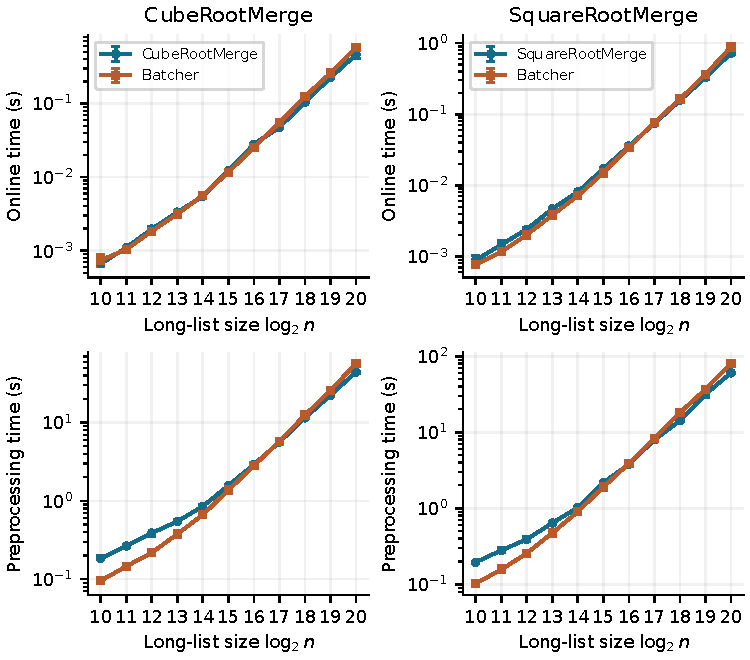
\includegraphics[width=\linewidth]{plots/root/root-merge-local.pdf}
\caption{Local online and preprocessing times for both asymmetric shapes.
Each marker is a three-run median with its observed range. Both parties
execute on one OS thread.}
\label{fig:root-local}
\end{figure}

\clearpage
\paragraph{Network sensitivity and preprocessing.}
We emulate LAN (1\,Gbit/s, 0.2\,ms RTT) and WAN (100\,Mbit/s, 40\,ms RTT)
links using isolated Linux network namespaces and a virtual Ethernet pair.
Each direction receives a \texttt{tc netem} rate limit and half the specified
RTT. Both endpoints run on this laptop. We take three matched executions
on both profiles at $n=2^{12}$ and $2^{16}$ and on WAN at $n=2^{20}$.
TCP phase time is the slower endpoint's time. Offline-plus-online time sums
these phase times per execution before taking the median.
An unloaded calibration measures mean RTTs of 0.270 and 40.597\,ms and
receiver TCP goodput of approximately 957 and 95.7\,Mbit/s for LAN and WAN,
respectively. The artifact retains the per-direction measurements and
interface offload settings.

At $n=2^{20}$, CubeRootMerge ($m=102$, $b=128$) sends 186.32\,MiB online versus 443.30\,MiB for matched Batcher, a 58.0\% reduction. Its local online median is 0.461\,s (range 0.415--0.466), versus 0.578\,s (0.573--0.608).
On the emulated WAN, the online medians are 13.199 and 25.139\,s, respectively (1.90$\times$ speedup). Including preprocessing, the medians are 90.91 and 87.11\,s.

At $n=2^{20}$, SquareRootMerge ($m=1024$, $b=512$) sends 275.25\,MiB online versus 622.44\,MiB for matched Batcher, a 55.8\% reduction. Its local online median is 0.724\,s (range 0.688--0.726), versus 0.886\,s (0.885--0.915).
On the emulated WAN, the online medians are 20.018 and 33.836\,s, respectively (1.69$\times$ speedup). Including preprocessing, the medians are 118.66 and 120.57\,s.



The online gains do not imply a uniform improvement in total time.
At $2^{20}$, CubeRootMerge's WAN total is higher than Batcher's, while the
observed total-time ranges for SquareRootMerge and Batcher overlap.
At $2^{12}$, SquareRootMerge is slower online on WAN despite communicating
fewer bytes: its greater depth dominates on this small, latency-sensitive case.
Figure~\ref{fig:root-network} retains these smaller-size comparisons.

\begin{figure}[!htbp]
\centering
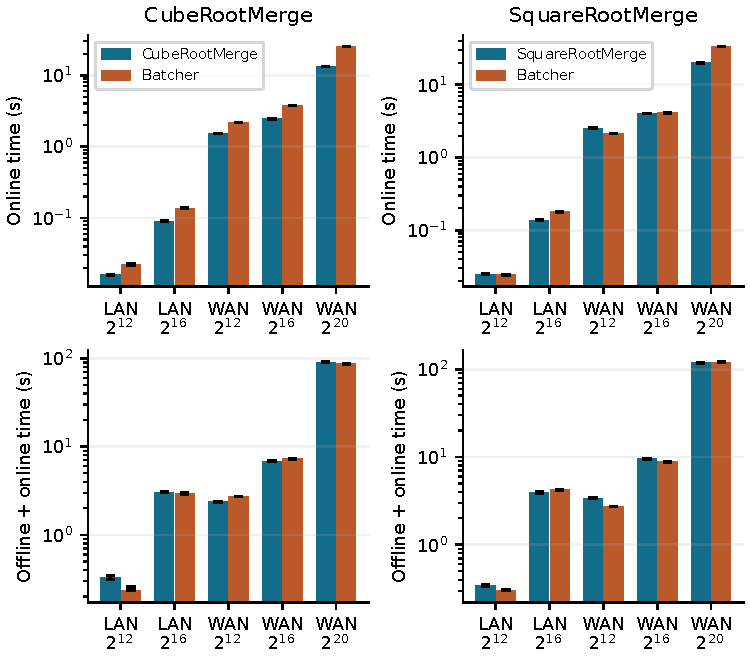
\includegraphics[width=\linewidth]{plots/root/root-merge-network.pdf}
\caption{Measured TCP online and offline-plus-online times for matched
asymmetric merges. Bars are three-run medians; error bars show observed
ranges. Rates are full-duplex caps per direction.}
\label{fig:root-network}
\end{figure}

Preprocessing generates GMW multiplication correlations and the two sets of
masked permutation correlations. Our online refinements do not remove the
permutation generator's OT/VOLE and PRF work. Accordingly, the artifact records
offline communication and time alongside every online measurement, as well as
peak memory and sampled swap. The implementation opportunities discussed in
Section~\ref{sec:packed-offline} also apply here; we make no quantitative claim
about unimplemented offline improvements. The raw records, selected parameters,
verification results, and plotting scripts are included in the artifact.
\clearpage
